\documentclass{article}
\usepackage{graphicx} % Required for inserting images
\usepackage{setspace} % Double Space 
\usepackage{ragged2e} % justify text
\usepackage{enumitem} % enumeration within subsection
\usepackage{url} % inserting links and urls

\usepackage{pdflscape} % Horizontal page orientation
\usepackage{booktabs}  % For \toprule, \midrule and \bottomrule
\usepackage{float} 

\usepackage[letterpaper, left=2cm, right=2cm, top=3cm, bottom=3cm]{geometry}

\setlength{\parskip}{1em} % we increase paragraph spacing

\title{Tesis}
\author{GUSTAVO ANDRES GONZALEZ PINEDA}
\date{February 2025}

\begin{document}

\begin{center}
\begin{doublespace}
    \thispagestyle{empty}  % no numbering for the cover
    \Large{UNIVERSIDAD DEL VALLE DE GUATEMALA}\\
    Facultad de Ingeniería \\
    Ingeniería en Ciencias de la Computación y Tecnologías de la Información 

    % Image placement
    \vspace{15mm} 
    
\includegraphics[width=0.2\textwidth]{images/Uvg_logo.jpg}

    \vspace{15mm} 
    {\Large Desarrollo de sistema de posicionamiento preciso en interiores mediante sensores UWB para recorridos virtuales con realidad aumentada en la Universidad del Valle de Guatemala.}

    \vspace{10mm} 
    {\Large Trabajo de graduación en modalidad de Trabajo Profesional presentado por Gustavo González
    para optar al grado academico de Licenciatura en Ingeniería en Ciencias de la Computación y Tecnologías de la Información.}

    {\Large Guatemala, \\ 2025}
    
\end{doublespace}
\end{center}

\newpage % page left purposely on blank

\thispagestyle{empty} % Remove headers and footers (optional)
\mbox{} % Ensure the page is not optimized away
\newpage % Move to the next page


\begin{center}
    \begin{doublespace}
        \thispagestyle{empty}  % no numbering for the cover
        \Large{UNIVERSIDAD DEL VALLE DE GUATEMALA}\\
        Facultad de Ingeniería \\
        Ingeniería en Ciencias de la Computación y Tecnologías de la Información 
    
        % Image placement
        \vspace{15mm} 
        
\includegraphics[width=0.2\textwidth]{images/Uvg_logo.jpg}
    
        \vspace{15mm} 
        {\Large  Desarrollo de sistema de posicionamiento preciso en interiores mediante sensores UWB para recorridos virtuales con realidad aumentada en la Universidad del Valle de Guatemala}
    
        \vspace{10mm} 
        {\Large Trabajo de graduación en modalidad de Trabajo Profesional presentado por Gustavo González
    para optar al grado academico de Licenciatura en Ingeniería en Ciencias de la Computación y Tecnologías de la Información.}
    
        {\Large Guatemala, \\ 2025}
        
    \end{doublespace}
    \end{center}


% end of cover section


\setcounter{page}{1} % Start page numbering from page 1

\section{Abstract}
{\justify This project aims to develop an augmented reality application for virtual tours within the campus of Universidad del Valle de Guatemala, integrating a precise navigation system using Estimote Beacons with Ultra-Wideband (UWB) technology. The solution seeks to improve orientation for students, visitors, and individuals with disabilities by facilitating movement between various campus locations through an interactive and accessible guide.

Unlike previous versions based on QR codes, this proposal leverages UWB to achieve more accurate and reliable positioning. The project includes campus mapping to strategically place sensors, the development of a communication architecture between mobile devices and the application built in Unity with AR Foundation, as well as the optimization of pathfinding algorithms—primarily A*—to generate efficient and adaptable routes in real time. This initiative represents a significant step forward in enhancing the university experience through the use of emerging technologies in localization and augmented reality.}

\section{Resumen}
{\justify Este proyecto tiene como objetivo desarrollar una aplicación de realidad aumentada para recorridos virtuales dentro del campus de la Universidad del Valle de Guatemala, integrando un sistema de navegación precisa mediante sensores Estimote Beacons con tecnología Ultra-Wideband (UWB). La solución busca mejorar la orientación de estudiantes, visitantes y personas con discapacidad, facilitando el desplazamiento entre distintos puntos del campus a través de una guía interactiva y accesible.

A diferencia de versiones previas basadas en códigos QR, esta propuesta utiliza UWB para lograr una localización más exacta y confiable. El proyecto abarca el mapeo del campus para ubicar estratégicamente los sensores, el desarrollo de una arquitectura de comunicación entre dispositivos móviles y la aplicación construida en Unity con AR Foundation, así como la optimización de algoritmos de pathfinding, principalmente A*, para generar rutas eficientes y adaptables en tiempo real. Esta iniciativa representa un avance significativo en la mejora de la experiencia universitaria mediante el uso de tecnologías emergentes en localización y realidad aumentada.}

\newpage

\section{Introducción}
{\justify
La orientación dentro de un campus universitario puede representar un desafío para estudiantes nuevos, visitantes y personas con
 discapacidad. Con el avance de la tecnología, la realidad aumentada (AR) se ha convertido en una herramienta innovadora para mejorar
  la experiencia de navegación en espacios físicos. En este contexto, el presente proyecto busca desarrollar una aplicación de realidad
   aumentada para recorridos dentro de la Universidad del Valle de Guatemala (UVG), proporcionando una guía interactiva e inclusiva 
   que facilite el desplazamiento desde un punto A hasta un punto B dentro del campus.

Este proyecto se basa en el trabajo realizado en años anteriores, donde se implementó una versión preliminar de la navegación con AR,
 pero con limitaciones significativas. Una de las principales dificultades fue la dependencia de códigos QR para la ubicación, lo que
  restringía la precisión y fluidez del recorrido. Además, la implementación del algoritmo de pathfinding presentaba problemas en la 
  generación de rutas óptimas, afectando la experiencia del usuario.

Para mejorar estos aspectos, la universidad ha invertido en sensores Estimote Beacons con tecnología Ultra-Wideband (UWB), los cuales
 permitirán una localización más precisa dentro del campus. La labor de este trabajo se centrará en el mapeo del campus para 
 determinar la ubicación óptima de estos sensores, su configuración e integración con la aplicación y la optimización del algoritmo
  de pathfinding para generar rutas más accesibles y eficientes.

El objetivo es mejorar la precisión de la navegación y evitar rutas poco prácticas o inaccesibles para ciertos usuarios. Esto 
contribuirá a una experiencia más fluida y efectiva al desplazarse dentro del campus, garantizando que la aplicación proporcione 
indicaciones precisas y usables en diferentes escenarios.A través de este trabajo, se espera ofrecer una solución innovadora y 
funcional que aproveche las capacidades de la realidad aumentada y la localización UWB para facilitar la movilidad dentro de la UVG,
 mejorando la orientación y accesibilidad dentro del campus universitario.}
\newpage

\section{Objetivos}
\subsection{Objetivo general}
{\justify Desarrollar e implementar un plugin de localización en tiempo real mediante sensores Estimote con tecnología Ultra-Wideband (UWB), integrado a Unity, como parte de una aplicación de realidad aumentada que facilite los recorridos virtuales dentro del Centro de Innovación y Tecnología (CIT) del campus de la Universidad del Valle de Guatemala.}

\subsection{Objetivos específicos}
\begin{enumerate}[label=\thesubsection.\arabic*]
    \item Diseñar e implementar un algoritmo de trilateración
para estimar la posición bidimensional del usuario dentro del campus universitario,
mediante el procesamiento de las distancias medidas hacia múltiples sensores Estimote UWB distribuidos en el entorno.
    \item Integrar el SDK nativo de Estimote para iOS con Unity
para permitir la obtención y transferencia en tiempo real de datos de localización hacia la aplicación de realidad aumentada,
mediante el desarrollo de un plugin nativo en Swift que sirva de puente entre ambas plataformas.
    \item Aplicar técnicas de filtrado de señales, como el filtro de Kalman
para mejorar la estabilidad del sistema de localización y reducir el efecto de ruido o jitter en las mediciones,
mediante la combinación de los datos obtenidos por trilateración y los registros del acelerómetro del dispositivo.
    \item Documentar exhaustivamente el desarrollo del sistema de localización
para asegurar su mantenibilidad, facilitar su futura extensión a dispositivos Android y permitir su continuidad por generaciones futuras,
mediante la elaboración de documentación técnica clara sobre la arquitectura del plugin, las decisiones de diseño y los procesos de integración.
    \item Evaluar cualitativamente la precisión y suavidad del sistema de localización
para validar su funcionamiento en condiciones reales y su aporte a la experiencia de usuario dentro de la aplicación,
mediante la observación directa del comportamiento del sistema y el análisis de las distribuciones de datos de posición obtenidas durante pruebas manuales.       
\end{enumerate}

\newpage
\section{Justificación}
{\justify
Actualmente, el proceso de orientación para estudiantes nuevos, visitantes y padres de familia dentro del campus universitario de la Universidad del Valle de Guatemala presenta diversas limitaciones. Tradicionalmente, el recorrido por las instalaciones es guiado por estudiantes o personal universitario, pero este se realiza una única vez —si es que se llega a realizar— lo cual suele ser insuficiente para que los usuarios recuerden rutas, espacios o servicios disponibles. Como consecuencia, durante los primeros semestres, muchos estudiantes enfrentan dificultades para ubicarse, llegando a perderse o desaprovechar recursos valiosos del campus.

Además de la desorientación inicial, existen barreras de accesibilidad que afectan a personas con movilidad reducida o con discapacidades visuales, quienes podrían beneficiarse significativamente de un sistema que les permita planificar sus trayectos de forma precisa y adaptada a sus necesidades. Una solución tecnológica puede contribuir a solventar ambos problemas, mejorando tanto la orientación como la inclusión dentro del entorno universitario.

En este contexto, el desarrollo de una aplicación de realidad aumentada con capacidades de localización y navegación precisa representa una oportunidad para aplicar conocimientos técnicos adquiridos a lo largo de la carrera de Ingeniería en Ciencias de la Computación y Tecnologías de la Información. Este proyecto integra áreas clave como programación orientada a objetos, interacción humano-computadora, gráficos por computadora, desarrollo móvil y algoritmos de búsqueda de caminos (pathfinding). Asimismo, se utilizarán sensores Estimote Beacons con tecnología Ultra-Wideband (UWB), cuya precisión y facilidad de conexión brindan una ventaja considerable en comparación con tecnologías previamente utilizadas, como los códigos QR.

Este trabajo, al ser parte de un megaproyecto en curso, busca fortalecer y mejorar la versión previa de la aplicación desarrollada por generaciones anteriores, proponiendo avances significativos en la precisión de la localización y en la experiencia del usuario. La solución no solo resolverá problemas existentes, sino que también funcionará como base tecnológica para futuras generaciones de estudiantes que podrán continuar desarrollando y afinando la herramienta.

Finalmente, este proyecto aporta a la universidad al fortalecer su imagen como institución innovadora, capaz de generar soluciones tecnológicas útiles y vanguardistas dentro de su propio entorno. Comunica el potencial de sus estudiantes para abordar problemas reales mediante el uso creativo y riguroso del conocimiento adquirido, posicionando a la UVG como una universidad comprometida con la tecnología, la accesibilidad y la experiencia estudiantil.}

\newpage
\section{Marco Teórico}
\subsection{Localización en interiores}
{\justify La localización en interiores, también conocida como Indoor Positioning, es un área de estudio dentro de la computación ubicua que busca determinar la posición de personas u objetos dentro de espacios cerrados, donde las señales satelitales como el GPS pierden cobertura o presentan alta inexactitud. A diferencia de los sistemas de localización en exteriores, la implementación de soluciones en interiores implica múltiples retos técnicos, como la interferencia de estructuras físicas (paredes, techos, mobiliario), el comportamiento impredecible de las señales de radiofrecuencia por efectos como la reflexión, refracción y difracción, así como la variabilidad en el entorno.

Para suplir estas limitaciones, se han explorado diferentes tecnologías de localización alternativas, entre ellas Wi-Fi, Bluetooth Low Energy (BLE), RFID, visión por computadora y Ultra-Wideband (UWB). Cada tecnología ofrece un compromiso distinto entre precisión, consumo energético, costo y complejidad de implementación. En entornos que requieren alta precisión —como hospitales, bodegas o, en este caso, instalaciones universitarias complejas—, el UWB se destaca por ofrecer ventajas clave frente a sus competidores, sobre todo en términos de exactitud, latencia y robustez frente al ruido ambiental.}


\subsection{Tecnología Ultra-Wideband (UWB)}
{\justify La tecnología Ultra-Wideband (UWB) se basa en el uso de pulsos de muy corta duración que se propagan en un espectro extremadamente amplio (mayor a 500 MHz). Esta característica permite transmitir datos con alta precisión temporal, lo que a su vez facilita la medición del tiempo exacto que tarda una señal en desplazarse entre dos dispositivos. A través de estos tiempos de vuelo (Time of Flight, ToF), un receptor puede estimar con mucha precisión la distancia a un emisor, sin depender de la intensidad de la señal (RSSI), como ocurre en tecnologías menos precisas como BLE o Wi-Fi.

En aplicaciones de localización, los dispositivos UWB se colocan en el entorno como anclas o beacons, que transmiten pulsos periódicamente. Un dispositivo móvil equipado con un receptor UWB puede calcular su distancia a múltiples beacons y usar dicha información para estimar su posición. Esta técnica, que combina alta precisión (en el orden de decímetros o incluso centímetros) con baja latencia, es ideal para aplicaciones donde se requiere posicionamiento en tiempo real con gran fidelidad espacial, como la navegación asistida con realidad aumentada. En este proyecto se utilizan sensores Estimote UWB Beacons, diseñados específicamente para tareas de localización en interiores, con soporte en plataformas móviles como iOS.}


\subsection{Trilateración}
{\justify La trilateración es un método geométrico fundamental en sistemas de localización que permite calcular la posición de un punto desconocido en el espacio utilizando las distancias conocidas a tres o más puntos de referencia cuyas ubicaciones son fijas. En el caso de localización en dos dimensiones, si se conocen las coordenadas de tres sensores (beacons) y las distancias del dispositivo móvil a cada uno de ellos, es posible determinar su posición mediante la intersección de los tres círculos generados por esas distancias. En la práctica, debido a errores de medición, estas circunferencias rara vez se intersectan en un solo punto, por lo que se recurre a métodos de optimización y regresión para encontrar el punto más probable.

Cuando se disponen más de tres sensores, se puede aplicar trilateración redundante, técnica que permite mejorar la estabilidad de la estimación al reducir el impacto de errores individuales en las mediciones. La trilateración es la base matemática de muchos sistemas de localización, incluidos GPS, y en este proyecto, se adapta al contexto del campus universitario, utilizando coordenadas cartesianas en un plano 2D para determinar la ubicación del usuario en tiempo real.}

\subsection{ Filtro de Kalman}
{\justify El filtro de Kalman es un algoritmo recursivo de estimación desarrollado por Rudolf E. Kálmán en la década de 1960, utilizado para predecir el estado de un sistema dinámico y corregir esa predicción a partir de mediciones ruidosas. Su aplicación ha sido clave en campos como la navegación inercial, la robótica, el seguimiento de objetos y los sistemas de control, debido a su capacidad para integrar múltiples fuentes de información en presencia de incertidumbre.

En el contexto de este proyecto, el filtro de Kalman se emplea para suavizar la trayectoria estimada del usuario dentro del campus, combinando las posiciones calculadas mediante trilateración con los datos del acelerómetro del dispositivo móvil. Esta fusión sensorial permite reducir el jitter, es decir, las pequeñas oscilaciones aleatorias en la posición del usuario, y mejorar la estabilidad de la trayectoria percibida. Aunque el sistema no busca una precisión milimétrica absoluta, el objetivo es proporcionar una experiencia de navegación fluida, donde la posición calculada varíe de forma coherente con el movimiento del usuario.}

\subsection{Acelerómetro}
{\justify El acelerómetro es un sensor electrónico capaz de medir la aceleración de un cuerpo en los tres ejes del espacio (x, y, z), tanto por efecto del movimiento como por la fuerza gravitacional. En los dispositivos móviles modernos, los acelerómetros permiten funciones como la detección de orientación, el conteo de pasos, y la navegación sin GPS (dead reckoning).

En este proyecto, el acelerómetro se utiliza como complemento a la trilateración UWB para mejorar la estimación de la posición del usuario. Aunque los acelerómetros presentan el inconveniente de la deriva acumulativa (pequeños errores que se amplifican con el tiempo cuando se integra la aceleración), su uso combinado con los datos de distancia de los sensores UWB, mediante el filtro de Kalman, permite detectar transiciones suaves en el movimiento del usuario, anticipar su dirección y estabilizar la trayectoria. De esta manera, el sistema puede ofrecer una experiencia más coherente y natural en la navegación con realidad aumentada.}

\subsection{Unity y Realidad Aumentada}
{\justify Unity es un motor de desarrollo multiplataforma ampliamente utilizado en la industria de los videojuegos, simulaciones y aplicaciones interactivas. Su compatibilidad con dispositivos móviles y su integración con librerías de realidad aumentada como ARKit (iOS) y ARCore (Android), lo convierten en una herramienta poderosa para el desarrollo de experiencias inmersivas en tiempo real.

En este proyecto, Unity se emplea como el entorno de ejecución principal para la aplicación de recorridos virtuales con realidad aumentada. A través de la cámara del dispositivo móvil, el usuario puede observar su entorno mientras el sistema le sobreimpone elementos gráficos —como flechas tridimensionales— que le indican hacia dónde debe avanzar para completar un recorrido. La interacción entre estos elementos visuales y el sistema de localización precisa permite convertir el espacio físico del campus en una experiencia guiada interactiva, intuitiva y accesible.}

\subsection{Plugins Nativos para Unity (iOS)}
{\justify Debido a que Unity no ofrece acceso directo a todas las funcionalidades del sistema operativo, como sensores especializados o bibliotecas nativas, es común extender su funcionalidad mediante plugins nativos. Un plugin nativo permite conectar el código de Unity con código escrito en lenguajes como Swift (para iOS) o Kotlin (para Android), habilitando el uso de SDKs que solo están disponibles de forma nativa.

En el caso de este proyecto, se desarrolla un plugin en Swift que se encarga de establecer la comunicación con los sensores Estimote UWB, procesar las mediciones de distancia, acceder a los datos del acelerómetro mediante el framework CoreMotion, realizar los cálculos de trilateración y aplicar el filtro de Kalman. Este plugin se comunica con Unity a través de una interfaz de funciones expuestas, enviando las coordenadas calculadas para ser usadas por el motor gráfico en la navegación. Esta arquitectura modular garantiza que el sistema pueda mantenerse y extenderse fácilmente, incluyendo la posibilidad futura de implementar un plugin análogo para Android.}


\section{Metodología}
\subsection{Introducción}

Para alcanzar los objetivos planteados en este proyecto, se ha diseñado una metodología de carácter \textbf{experimental} que combina conocimientos de programación, redes, sensores y realidad aumentada. La implementación se divide en fases que abordan el mapeo del campus, la integración de sensores y la navegación por medio de un sistema de realidad aumentada.

\subsection{Tipo de investigación}

La investigación realizada es de tipo \textbf{experimental}, ya que se basa en la prueba, validación y ajuste continuo de tecnologías y algoritmos en un entorno real. Esto permite adaptar las soluciones conforme se identifican oportunidades de mejora durante el desarrollo.

\subsection{Metodología estructurada por objetivos}

\subsubsection{Objetivo 1: Realizar el mapeo de la universidad para determinar la ubicación óptima de los sensores Estimote Beacons con tecnología UWB}

\begin{itemize}
    \item \textbf{Fase 1: Análisis del entorno} \\
    Se utilizará un modelo 3D ya existente del campus, previamente construido con base en planos oficiales y validado manualmente.

    \item \textbf{Fase 2: Planificación de distribución} \\
    Se propondrá una distribución preliminar de los sensores siguiendo un patrón en zigzag, buscando una cobertura eficiente. Esta hipótesis será validada mediante pruebas de campo.

    \item \textbf{Fase 3: Validación de ubicación} \\
    Se colocarán sensores físicamente en puntos estratégicos y se realizarán pruebas de señal para determinar la calidad y precisión. Se explorarán configuraciones alternativas si los resultados no son satisfactorios.
\end{itemize}

\textit{Herramientas y conocimientos aplicados:} propagación de señales, redes inalámbricas, análisis espacial.

\subsubsection{Objetivo 2: Configurar e integrar los sensores Estimote Beacons en la aplicación de realidad aumentada}

\begin{itemize}
    \item \textbf{Fase 1: Lectura y conexión de sensores} \\
    Se implementarán módulos nativos para Android e iOS capaces de conectarse con los Estimote Beacons utilizando sus respectivos SDKs.

    \item \textbf{Fase 2: Comunicación entre módulos y Unity} \\
    Debido a que el SDK de los sensores UWB sólo está disponible para plataformas nativas (iOS o Android), se ha optado por una arquitectura basada en \textbf{plugins nativos para Unity}. Estos plugins permiten que el código nativo, encargado de la conexión con los sensores, pueda interactuar con Unity.

    El flujo de datos contempla dos posibles alternativas que se evaluarán según rendimiento:
    \begin{itemize}
        \item Procesar la trilateración y manejo de sensores de forma nativa y luego enviar los resultados (posición estimada) a Unity mediante el plugin.
        \item Enviar los datos crudos (como señales o distancias) a Unity a través del plugin y realizar el procesamiento dentro de Unity.
    \end{itemize}

    Se elegirá la opción más eficiente en función de pruebas de rendimiento y facilidad de integración. Posteriormente, una vez se tenga la posición estimada del usuario, se utilizará \textbf{ARFoundation de Unity} para presentar los elementos en realidad aumentada de forma sincronizada con el entorno físico.

    Además, se aprovecharán los sensores del dispositivo móvil como el \textbf{giroscopio} para complementar los datos recibidos de los sensores UWB, mejorando la precisión y la experiencia del usuario final, especialmente en escenarios donde exista latencia o pérdida temporal de señal.

    \item \textbf{Fase 3: Complementación con sensores del dispositivo} \\
    Se combinará la información de los beacons con los datos del giroscopio del dispositivo móvil para mejorar la precisión de la localización y suavizar la experiencia del usuario en caso de latencias.
\end{itemize}

\textit{Herramientas y conocimientos aplicados:} programación de plataformas móviles, interacción entre capas nativas y motores gráficos, fundamentos de sensores y microprocesadores.

\subsubsection{Objetivo 3: Optimizar el algoritmo de pathfinding para generar rutas accesibles y mejorar la experiencia del usuario}

\begin{itemize}
    \item \textbf{Fase 1: Definición del grafo de navegación} \\
    Se colocarán nodos clave dentro del modelo 3D del campus para representar ubicaciones importantes. Estos nodos y sus conexiones formarán el grafo utilizado para el pathfinding.

    \item \textbf{Fase 2: Implementación del pathfinding} \\
    Inicialmente se utilizará el módulo de navegación de Unity. Si los resultados no son óptimos, se evaluarán alternativas como A* o Dijkstra.

    \item \textbf{Fase 3: Evaluación de rendimiento} \\
    Se medirán tiempos de cálculo, uso de memoria, consumo de CPU y tiempos de respuesta. Se prioriza la experiencia fluida del usuario mediante la sincronización entre su movimiento y la visualización de rutas.
\end{itemize}

\textit{Herramientas y conocimientos aplicados:} estructuras de datos, optimización de algoritmos, Unity Navigation, AR Foundation.

\subsection{Recolección de datos}

Los datos a recolectar incluyen:

\begin{itemize}
    \item Distancia estimada entre usuario y sensores (medida directamente o inferida por intensidad de señal).
    \item Datos de orientación y desplazamiento proporcionados por el giroscopio del dispositivo móvil.
    \item Tiempos de respuesta de sensores y eficiencia del sistema de navegación.
    \item Precisión de localización comparando posición estimada con posición real.
\end{itemize}

Las pruebas se realizarán de forma interna y controlada dentro del campus utilizando distintos dispositivos compatibles.

\subsection{Análisis de datos}

Los datos recolectados serán analizados para:

\begin{itemize}
    \item Evaluar precisión de localización.
    \item Comparar rendimiento entre diferentes configuraciones.
    \item Validar la integración del sistema bajo condiciones reales de uso.
\end{itemize}

Se utilizarán herramientas como \textit{profilers} de Unity, logs del sistema y pruebas de campo.

\subsection{Consideraciones éticas}

Aunque esta fase del proyecto no implica interacción directa con usuarios reales, en etapas futuras se deberá:

\begin{itemize}
    \item Obtener consentimiento informado.
    \item Proteger la privacidad de los datos de localización.
    \item Ser transparentes en el uso de la información recolectada.
\end{itemize}

Actualmente, todos los datos utilizados son técnicos y se obtienen mediante pruebas internas controladas.

\newpage

\section{Cronograma}

% Image placement
\vspace{15mm} 
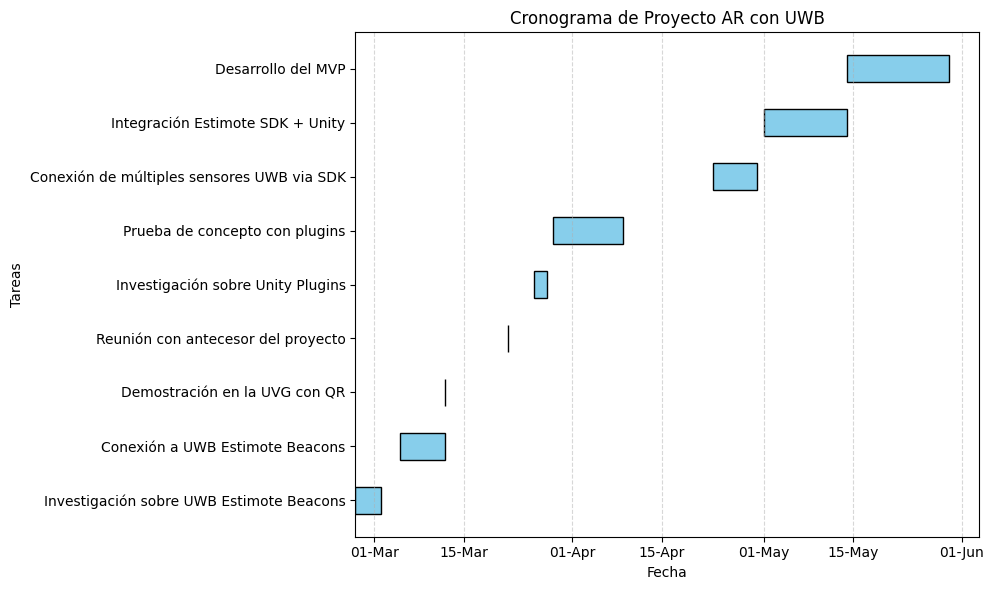
\includegraphics[width=1\textwidth]{images/cronograma.png}
{\begin{center}
    Figura 1: Cronograma del proyecto para el primer semestre.
\end{center}}
\newpage

    
 

\section{Bibliografía}
\begin{itemize} 
    % Bibliografia del marco teorico
    \item  Estimote, Inc. (n.d.). Estimote Proximity SDK. Estimote Documentation. Recuperado de: \url{https://developer.estimote.com/proximity/android-tutorial/}
    
    \item Estimote, Inc. (n.d.). Estimote Location Beacons: UWB and BLE. Estimote Documentation. Recuperado de: \url{https://developer.estimote.com/proximity/ultra-wideband/}
	
	\item Unity Technologies. (n.d.). AR Foundation overview. Unity Documentation. Recuperado de: \url{https://docs.unity3d.com/Packages/com.unity.xr.arfoundation@5.0/manual/index.html}
	
	\item Unity Technologies. (n.d.). Unity Manual: ARKit and ARCore with AR Foundation. Recuperado de: \url{https://docs.unity3d.com/Manual/com.unity.xr.arfoundation.html}
	
	\item Hart, P. E., Nilsson, N. J., \& Raphael, B. (1968). A formal basis for the heuristic determination of minimum cost paths. IEEE Transactions on Systems Science and Cybernetics, 4(2), 100–107. \url{https://doi.org/10.1109/TSSC.1968.300136}
	
	\item Thrun, S., Burgard, W., \& Fox, D. (2005). Probabilistic Robotics. MIT Press.
	
	\item Google. (n.d.). Bluetooth Low Energy overview | Android Developers. Recuperado de: \url{https://developer.android.com/guide/topics/connectivity/bluetooth-le}
	
	\item Apple Inc. (n.d.). Core Bluetooth Overview. Recuperado de: \url{https://developer.apple.com/documentation/corebluetooth}
\end{itemize}

\end{document}